\begin{figure}[t] \centering 
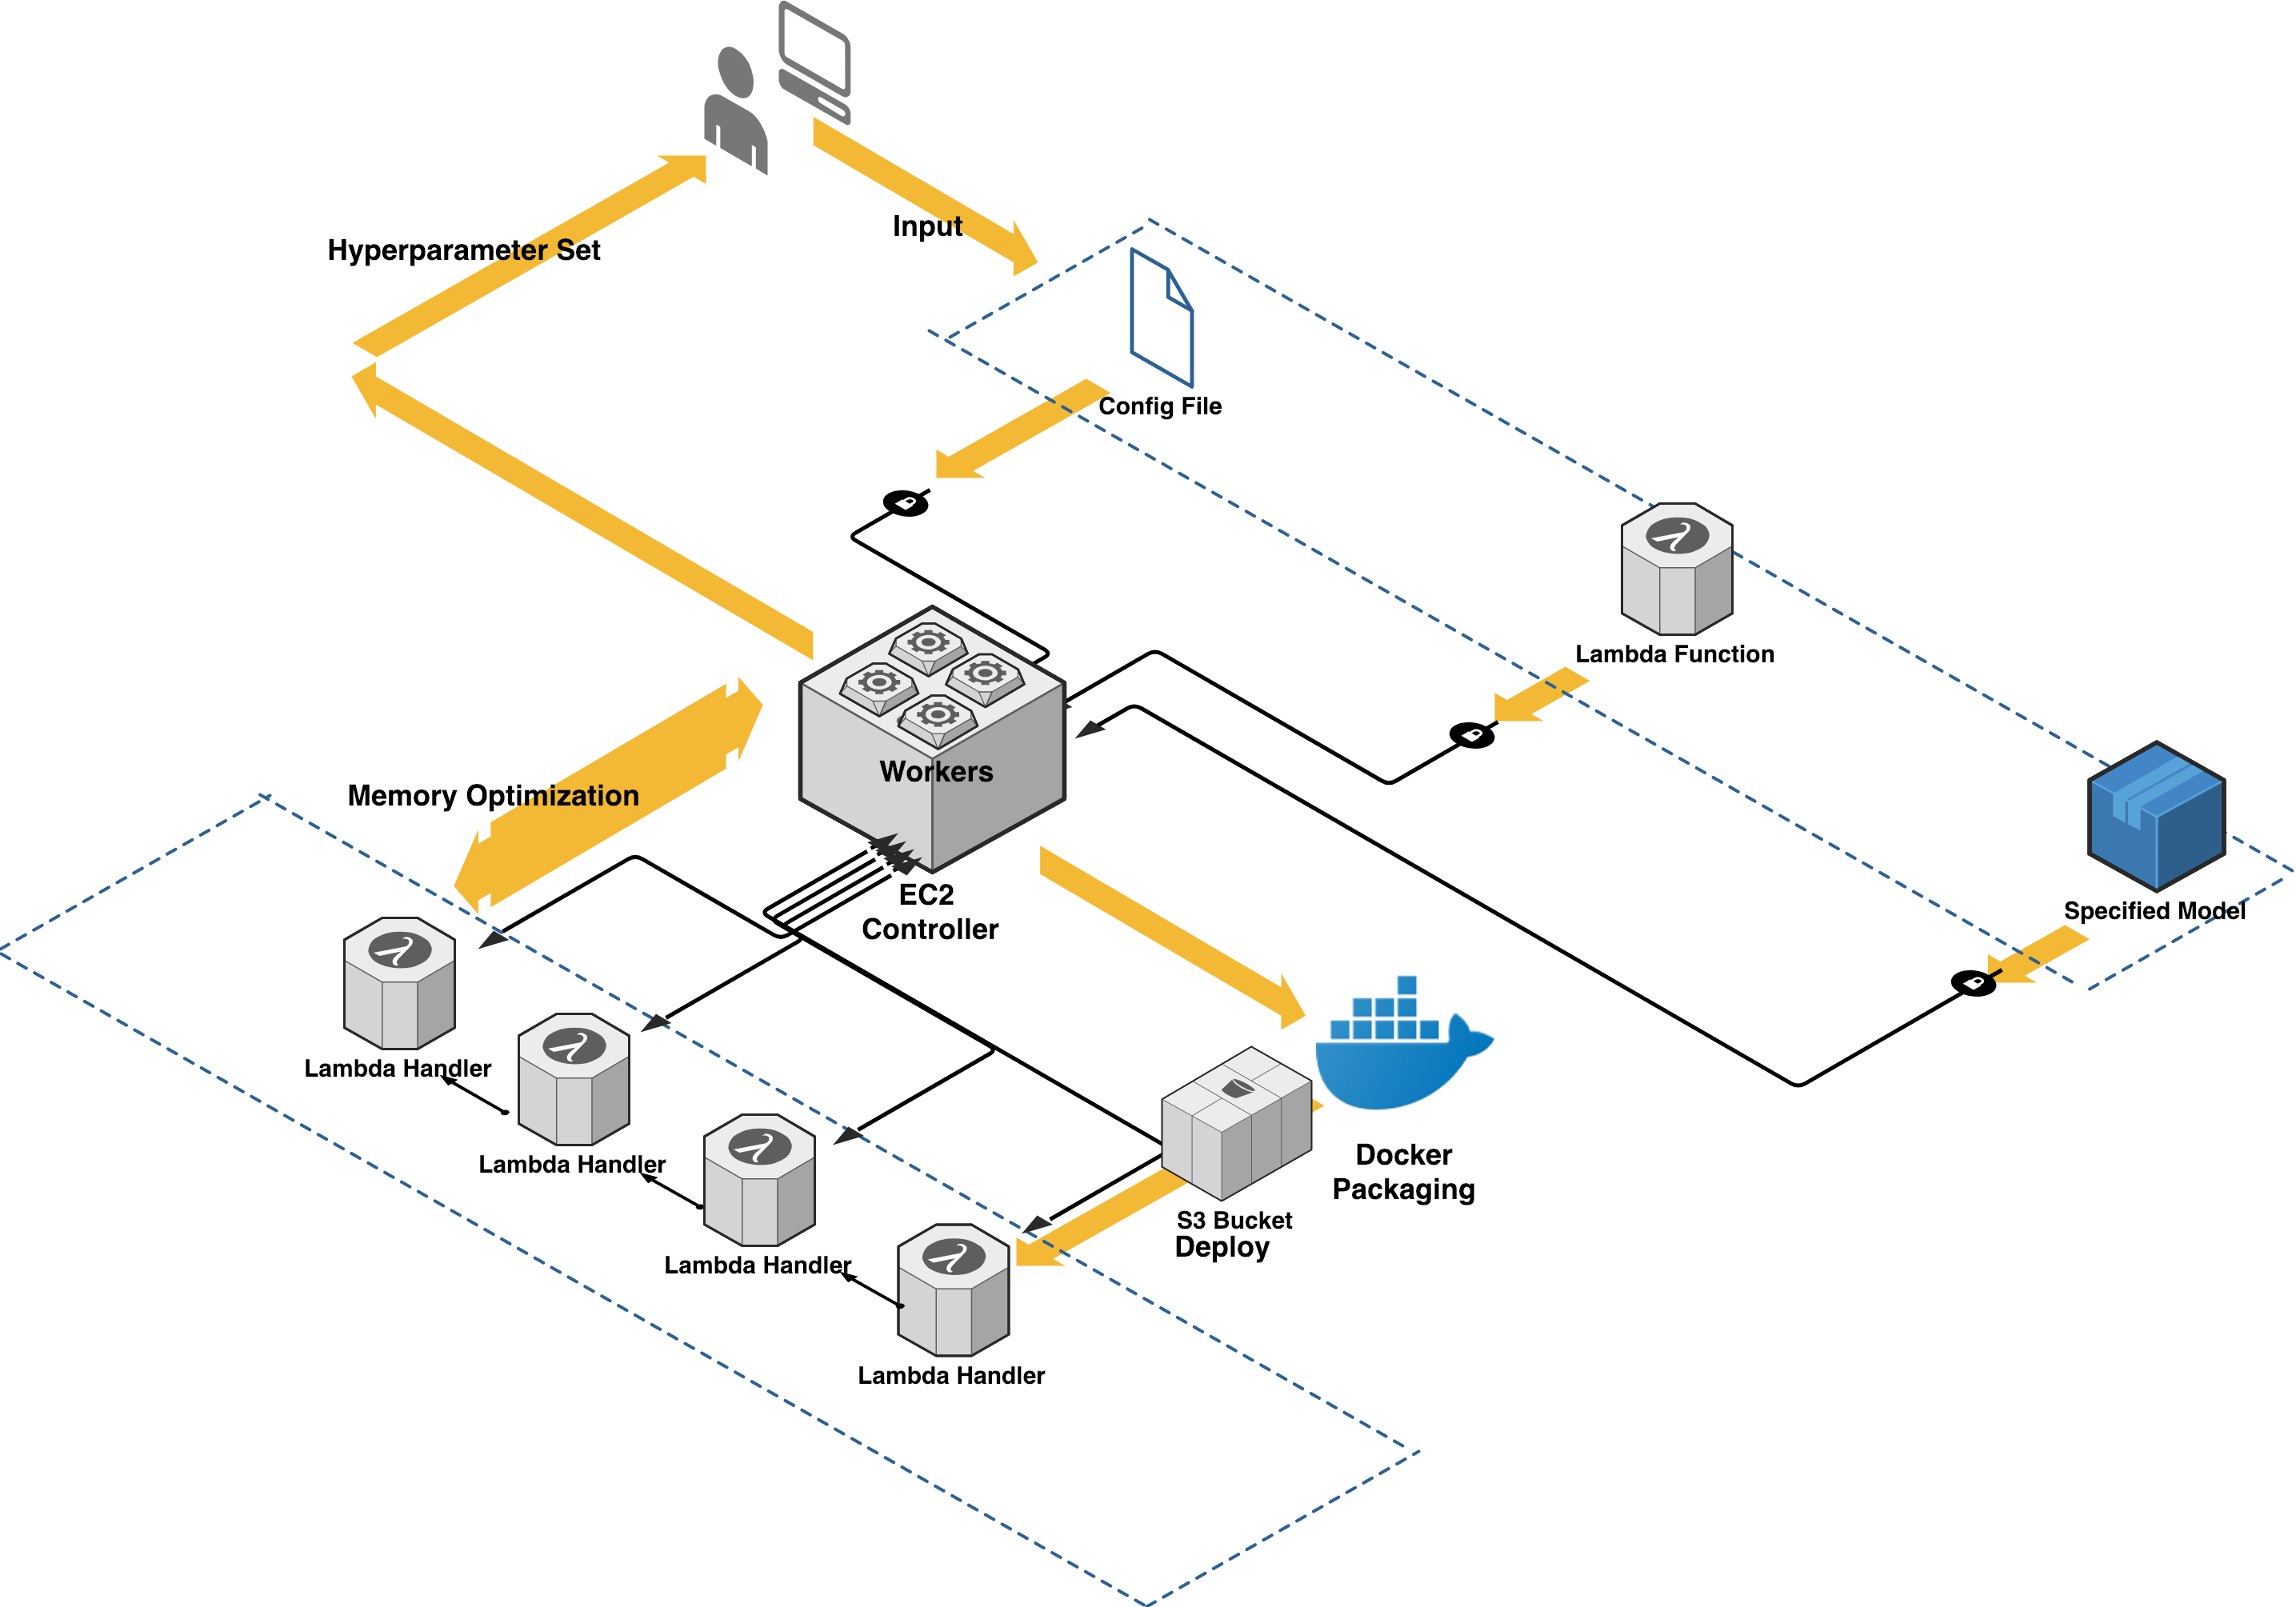
\includegraphics[scale=0.08]{Seneca}
\caption{The Seneca Architecture.
%Users specify hyperparameter options in the configuration file and provides lambda function. Seneca automatically package, deploy and optimize lambda function on AWS before completing grid search process and selecting best hyperparameter setting.
\label{fig:seneca}}
\vspace{-0.2in}
\end{figure}

To facilitate model search and selection using the serverless
architecture, we have developed Seneca, a framework for tuning the
hyperparameters of machine learning applications in AWS Lambda.  The
Seneca pipeline consists of packaging, deployment, function
optimization, and hyperparameter tuning. Figure~\ref{fig:seneca} shows
the architecture of Seneca.  In the the upper-right-front, we show the
three inputs that Seneca expects from its users: (\textit{A}) a
hyperparameter configuration file, (\textit{B}) a dataset URL, and
(\textit{C}) the lambda function of the machine learning
application. The configuration file specifies a set of values for
each hyperparameter that the application expects. Seneca creates the
Cartesian product of all options in this configuration as
the search space. The dataset URL refers to a valid dataset stored in
the AWS Simple Storage Service (S3)~\cite{ref:awss3}.
%\footnote{\url{https://aws.amazon.com/s3/}}.

Based on the specified machine learning application, Seneca
automatically builds and deploys an AWS Lambda application by
launching a Docker container that mirrors the AWS Lambda execution
environment, checks and installs the machine learning application and
any libraries it requires, compresses the application and uploads it
to S3 (a
work-around for the 10MB AWS Lambda function size restriction).
Seneca constructs an AWS Lambda function from a template that, when
executed, will download the dataset and split it into a training and
testing set, and construct, test, and evaluate a model using the
application and a set of hyperparameter values passed in by Seneca as
arguments.  Users can specify the train/test split ratio that should
be used by Seneca; the default is 80\%/20\%.  The function returns a
testing score.  Upon completion of this process, the container deploys
the function to AWS Lambda using the AWS Command Line
Interface~\cite{ref:awscli}
%\footnote{\url{https://aws.amazon.com/cli/}} 
and the developers credentials.



\subsection{Optimizing Memory Use}

The cost of using AWS Lambda (i.e. \texttt{compute charge}) 
is the billed duration (execution time rounded up to the
nearest 100ms)~\cite{ref:pricing}
%~\footnote{\url{https://aws.amazon.com/lambda/pricing/}}
multiplied by the allocated memory of each invoked function.
One goal of our work is to optimize memory use of these
applications in order to reduce cost, and to investigate
the trade-offs of doing so.

Currently, allocated memory for a Lambda function can be set
from 128MB to 3008MB in increments of 64MB.
AWS documentation~\cite{ref:lambdalimits}
%~\footnote{\url{https://docs.aws.amazon.com/lambda/latest/dg/resource-model.html}} 
states that Lambda allocates CPU to functions  corresponding to allocated memory size,  
as is done for general purpose AWS EC2 instance types.

\begin{figure}[t] \centering 
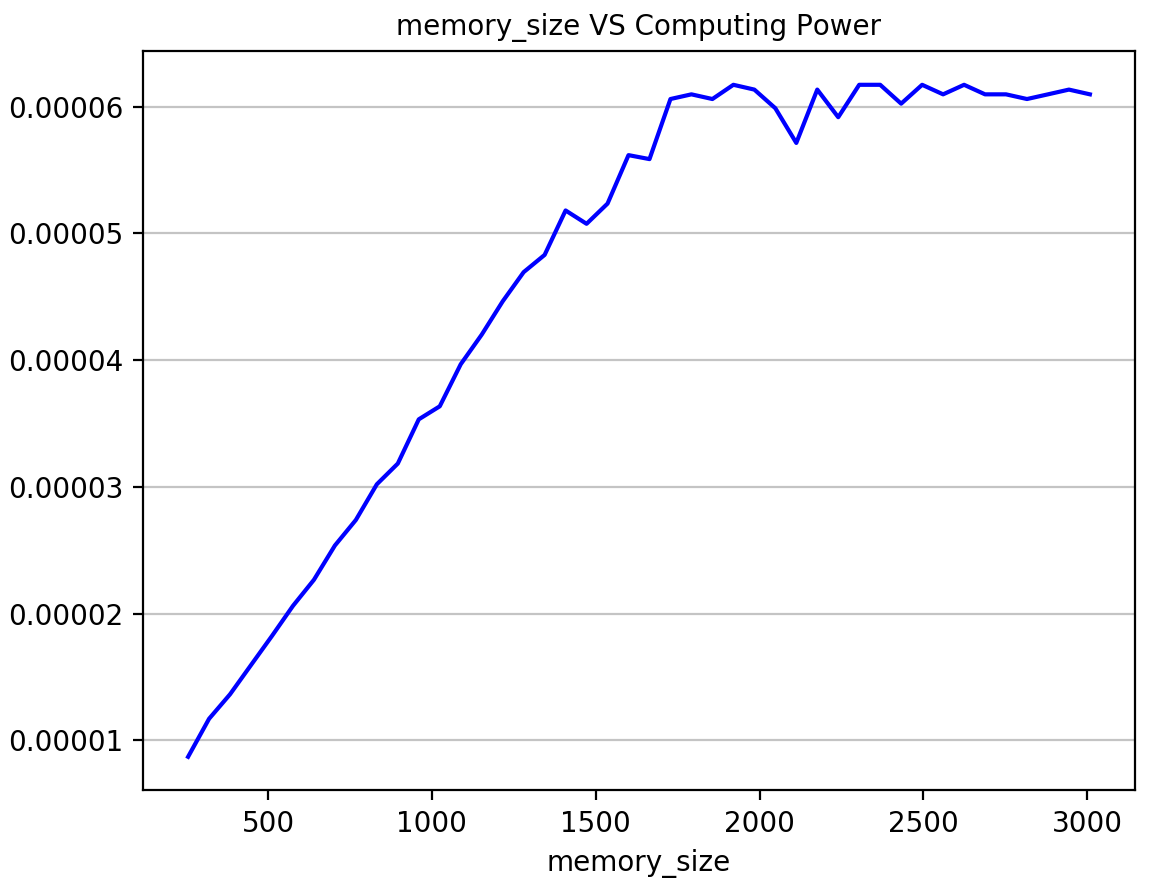
\includegraphics[scale=0.5]{memory}
\caption{The relationship between allocated memory and reciprocal of billed duration, which represents compute power for a compute-bound Lambda function.
\label{fig:memory}}
% \vspace{-0.2in}
\end{figure}

\begin{figure}[t] \centering 
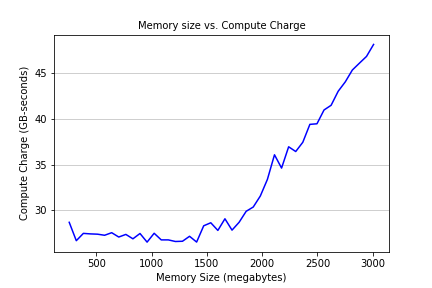
\includegraphics[scale=0.5]{compute_charge}
\caption{The relationship between allocated memory and compute charge for a compute-bound Lambda function.
\label{fig:compute_charge}}
% \vspace{-0.2in}
\end{figure}


To evaluate the relationship between memory, CPU, and cost, 
we analyze a 3-D matrix multiplication serverless benchmark~\cite{ref:matrix} using AWS Lambda.
We configure different functions to use each of the 46 possible allocated memory 
options.  Figure~\ref{fig:memory} shows the relationship between allocated memory 
(x-axis) and reciprocal of billed duration (y-axis). 
Figure~\ref{fig:compute_charge} shows the relationship between memory 
size (x-axis) and compute charge (y-axis). 
We observe that for this benchmark, billed duration 
plateaus after 1600 MB, at which point compute charge increases.
That is, we achieve no further execution time benefit (only cost increase)
after this point.

We use this relationship within
Seneca to optimize its cost (\texttt{compute charge}) via an extension
that enables it to automatically identify the appropriate
setting for allocated memory for each application.
However, instead of exhaustively testing all 46 possible 
memory configurations as we did for the matrix benchmark, 
which may be costly,  Seneca employs the heuristic outlined in
Algorithm~\ref{algo:optimizer}. 

The Seneca optimizer first configures and invokes the function using a user-defined payload.  From this run, Seneca obtains the \texttt{maximum memory used}
by the function as reported by AWS Cloudwatch,
and uses it as the starting point in its search.
Seneca then defines two double-ended queues 
(\textit{deque}) of length N, to store 
\texttt{allocated memory} and \texttt{compute charge} data of different invocations. While the current 
allocated memory is less than or equal to 3008 MB, 
the optimizer reconfigures and invokes the function 
using the next increment for memory allocation.  It 
calculates the compute charge for each invocation 
using current allocated memory and billed duration. 

We employ two exit conditions. The first is when the  compute charge monotonically increases across \textit{deque}. The second is when the increase in slope is greater than a threshold. When the optimizer finds that both conditions hold, it pops the left-most value from \textit{deque} and configures the function to use that value for allocated memory for all future invocations. If these two conditions can not be satisfied during search, the allocated memory will be configured as the memory size that results in minimal compute charge within the \textit{deque}. After extensive experimentation, we find that $N=5$ and a slope threshold of 1 work best, but these values are configurable. In addition, this optimization can be turned on or off via a command line argument to Seneca.

\begin{algorithm}[]
\caption{Seneca Optimizer Heuristic}
\label{algo:optimizer}
\SetAlgoLined
\KwData{Typical payload}
\KwResult{Optimal allocated memory}
Find memory used by payload as starting point\;
Define deque for allocated memory \& compute charge\;
 \While{allocated memory $\leq$ 3008 MB}{
  \eIf{compute charge monotonically increases in deque \& slope $\geq$ threshold}{
   popleft from deque\;
   configure allocated memory as optimum\;
   exit()\;
   }{
   increase allocated memory by 64 MB\;
   probe lambda function\;
   append memory and compute charge to deque\;
  }
 }
\end{algorithm}

\subsection{Tuning Process}

To facilitate parallel function invocation, Seneca integrates 
Celery~\cite{ref:celery}.
%\footnote{\url{http://www.celeryproject.org/}}
Celery is an asynchronous task queue 
that uses distributed message passing. Celery workers are processes 
that take tasks from the queue, execute the tasks with the arguments specified, 
and store the result that is returned 
in a database (we use Redis~\cite{ref:redis}
%~\footnote{\url{https://redis.io/}} 
in our prototype). 

Based on the configuration file, Seneca creates and enqueues a list of
payloads (function arguments) for each combination of hyperparameter
values.  The Seneca celery workers invoke the application's Lambda
function by each payload for model construction. Upon function
termination, the worker records a score for the hyperparemeter
configuration in the database.  When the queue is drained and all
workers have completed, Seneca extracts and reports the best score,
configuration, and model from the database. Users can then use the
model for inference given other datasets without retraining to
amortize the time/cost of Seneca.
% Users can then evaluate the prediction power of the models (using Seneca if desired) 
% for other datasets without retraining to amortize the time/cost of Seneca.


We assume that the dataset supplied to Seneca by the user is representative of 
datasets on which the 
resulting model will be used.  In addition, we use prediction error as the 
score (i.e., mean squared error for regression and accuracy percentage for classification) 
instead of $R^2$, which describes explanatory power, to avoid overfitting.
As part of future work, we are considering using multiple datasets and a ranges
of hyperparameter values to preclude the need for users to specify
them and to consider a wider range of values.
